\subsubsection{設計思考}

\term{設計思考}{Design Thinking} は、必要や問題を理解し、それに対する解決策を考える思考である。設計対象はソフトウェアに限らない。建築、工業製品、組織、業務手順など、人が目的を持って作るものには設計が関わる。

ソフトウェア設計で重要なのは、問題と解決策を表す語彙を作ることである。ソフトウェアは、物理的な材料を削って作るものではなく、概念、名前、規則、手続き、データ、インタフェースを組み合わせて作る。したがって、設計は言語的な活動でもある。

設計思考は、次の五段階として理解できる。
\begin{enumerate}
  \item 目的や目標を明確にする。
  \item その目的を達成する概念的な構造を考える。
  \item 概念構造を実現する仕組みを考える。
  \item その仕組みを表し、利用するための記法や語彙を作る。
  \item 具体的な問題文脈で記法を使い、目的を達成する。
\end{enumerate}

\begin{definitionbox}
設計思考とは、問題を理解し、制約の中で複数の解決策を考え、根拠を持って選び、表現可能な形へまとめる思考である。
\end{definitionbox}

\begin{figure}[htbp]
\centering
\IfFileExists{assets/generated_figures/ch03/fig-ch03-02.png}{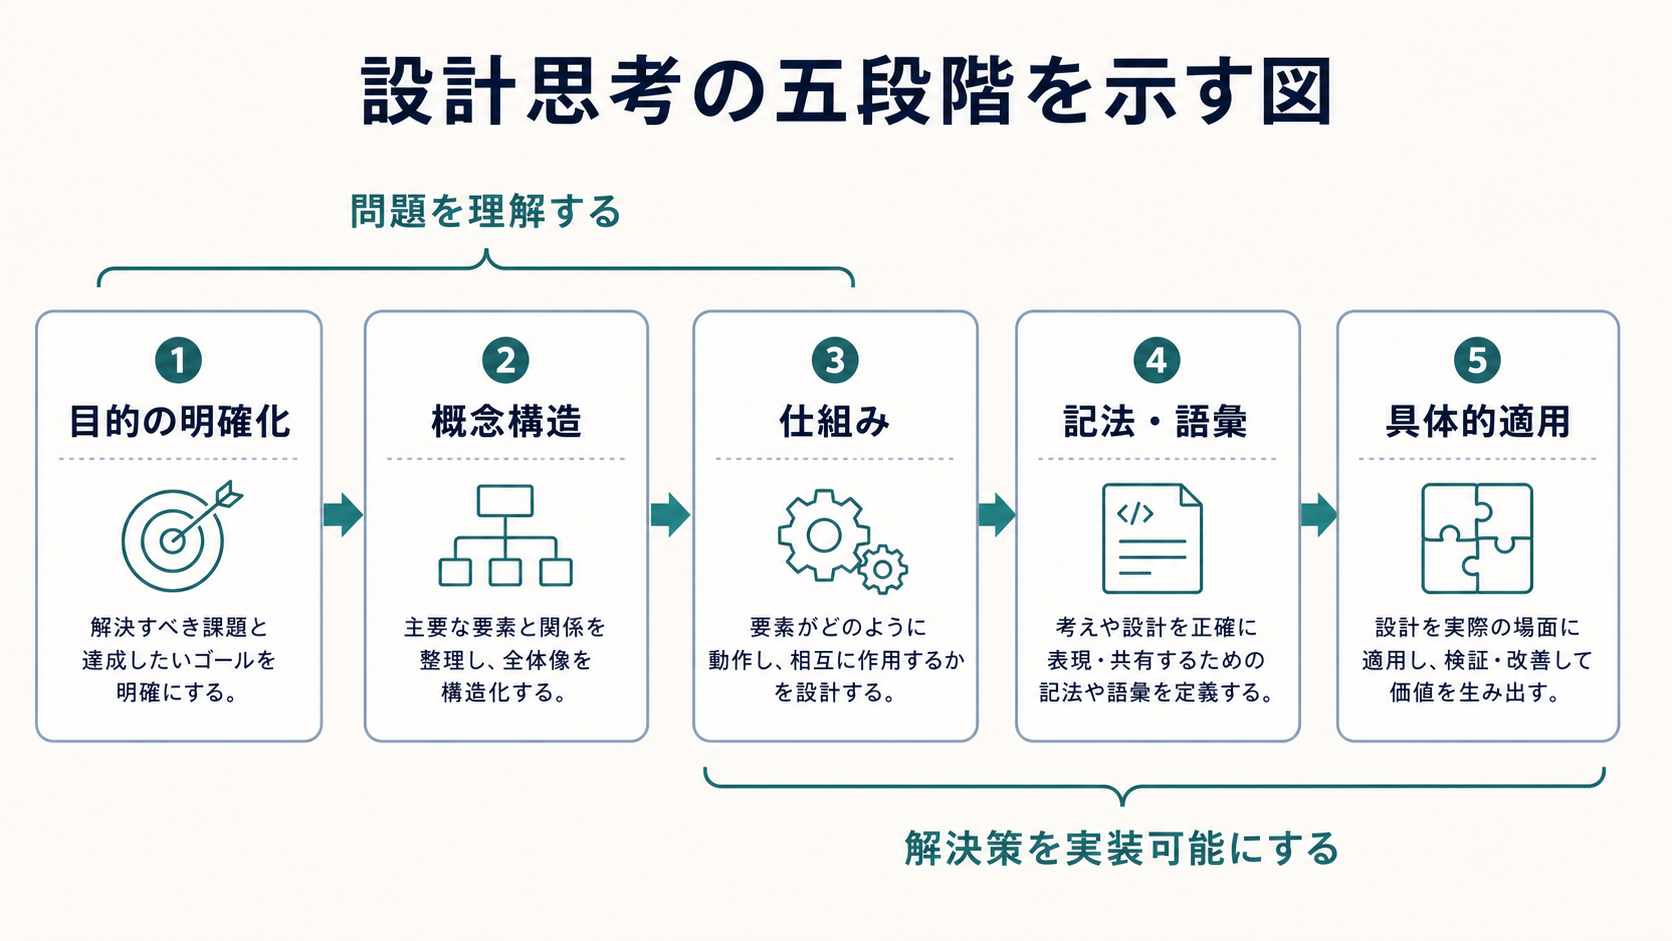
\includegraphics[width=0.96\linewidth]{assets/generated_figures/ch03/fig-ch03-02.png}}{\fbox{\parbox[c][48mm][c]{0.9\linewidth}{\centering 画像生成待ち\\設計思考の五段階を示す図}}}
\caption{設計思考の五段階を示す図}
\label{fig:ch03-02}
\end{figure}
